% !TeX program = xelatex
% AmSC Infrastructure for Agentic AI Workflows
% Audience: senior managers
% Build: xelatex amsc_agentic_ai.tex  (run twice)
\documentclass[aspectratio=169,11pt]{beamer}

\usetheme{metropolis}
\usepackage{fontspec}
\usepackage{graphicx}
\usepackage{tikz}
\usetikzlibrary{arrows.meta,positioning,shapes.geometric,fit,calc}
\usepackage{tcolorbox}
\tcbuselibrary{skins,breakable}
\usepackage{fontawesome5}
\usepackage{booktabs}
\usepackage{array}
\usepackage{listings}

% ---------------------------------------------------------------- palette
\definecolor{labnavy}{RGB}{18,42,73}
\definecolor{labink}{RGB}{40,44,52}
\definecolor{accentgold}{RGB}{223,161,54}
\definecolor{accentteal}{RGB}{0,137,123}
\definecolor{accentblue}{RGB}{41,98,168}
\definecolor{lightgray}{RGB}{245,246,248}
\definecolor{midgray}{RGB}{110,118,129}
\definecolor{okgreen}{RGB}{35,140,80}
\definecolor{softblue}{RGB}{215,228,248}
\definecolor{softteal}{RGB}{200,235,230}
\definecolor{softgold}{RGB}{250,235,200}
\definecolor{trinitypurple}{RGB}{90,72,200}
\definecolor{softtrinitypurple}{RGB}{235,232,255}

\setbeamercolor{background canvas}{bg=white}
\setbeamercolor{palette primary}{bg=labnavy,fg=white}
\setbeamercolor{frametitle}{bg=labnavy,fg=white}
\setbeamercolor{progress bar}{fg=accentteal,bg=lightgray}
\setbeamercolor{normal text}{fg=labink}
\setbeamercolor{alerted text}{fg=accentgold}
\setbeamercolor{footline}{fg=midgray}
\setbeamerfont{footline}{size=\tiny}
\setlength{\leftmargini}{14pt}

% ---------------------------------------------------------------- metadata
\newcommand{\deckauthor}{Huihuo Zheng}
\newcommand{\deckemail}{huihuo.zheng@anl.gov}
\newcommand{\deckinstitute}{Argonne Leadership Computing Facility (ALCF)}
\title{AmSC Infrastructure\\for Agentic AI Workflows}
\subtitle{IRI \textperiodcentered\ Globus Compute \textperiodcentered\ ClearML \textperiodcentered\ Trinity}
\date{August 2026}

% ---------------------------------------------------------------- logo
\newcommand{\decklogo}[1][0.16\textwidth]{%
  \IfFileExists{logos/argonne_logo.pdf}%
    {\includegraphics[width=#1]{logos/argonne_logo.pdf}}%
    {\textbf{\textsc{\textcolor{labnavy}{Argonne National Laboratory}}}}}
\logo{\IfFileExists{logos/argonne_logo.pdf}%
  {\includegraphics[height=0.42cm]{logos/argonne_logo.pdf}}{}}

% Trinity brand mark — overlay in the top-right corner (used on the Trinity slides)
\newcommand{\trinitymark}{%
  \IfFileExists{logos/trinity_logo.pdf}{%
    \begin{tikzpicture}[remember picture,overlay]
      \node[anchor=north east, inner sep=0pt]
        at ([xshift=-8pt,yshift=-3pt]current page.north east)
        {
\includegraphics[height=0.82cm]{logos/trinity_logo.pdf}};
    \end{tikzpicture}}{}}

% ---------------------------------------------------------------- shadowed boxes
\newtcolorbox{featbox}[2]{
  enhanced,
  colback=lightgray, colframe=#1, boxrule=0.6pt, arc=3pt,
  left=6pt, right=6pt, top=4pt, bottom=4pt,
  title=#2, colbacktitle=#1, coltitle=white,
  fonttitle=\bfseries\small, boxsep=1pt,
  halign title=flush left,
  drop fuzzy shadow
}
\newtcolorbox{calloutbox}[1][labnavy]{
  enhanced,
  colback=#1!6, colframe=#1, boxrule=0.6pt, arc=3pt,
  left=10pt, right=10pt, top=6pt, bottom=6pt,
  drop fuzzy shadow
}
% framed screenshot container (matches trinity_new_features style)
\newtcolorbox{shot}{%
  enhanced,colback=white,colframe=midgray!50,boxrule=0.5pt,arc=2pt,
  left=1.5pt,right=1.5pt,top=1.5pt,bottom=1.5pt,drop fuzzy shadow}
\newcommand{\shotcap}[1]{\par\vspace{2pt}{\scriptsize\itshape\color{midgray}#1}}
% italic section label inside a box
\newcommand{\subhead}[1]{\vspace{2pt}{\scriptsize\itshape\color{midgray}#1}\vspace{1pt}}

% ---------------------------------------------------------------- chat bubble + pill (from trinity_overview)
\newtcolorbox{chatbubble}[2]{
  enhanced,
  colback=#1!12, colframe=#1!60!black, boxrule=0.5pt, arc=5pt,
  left=8pt, right=8pt, top=3pt, bottom=3pt, width=\linewidth,
  title=#2, colbacktitle=#1!60!black, coltitle=white,
  fonttitle=\bfseries\footnotesize, boxsep=1pt,
  drop fuzzy shadow
}
\newcommand{\pill}[2]{\tikz[baseline=-0.5ex]{\node[draw=#1!70!black, fill=#1!12,
  rounded corners=3pt, inner sep=4pt, font=\bfseries\scriptsize] {#2};}}

% ---------------------------------------------------------------- shell listing style
\lstdefinestyle{shell}{
  language=bash,
  basicstyle=\ttfamily\scriptsize\color{labink},
  keywordstyle=\color{accentblue}\bfseries,
  commentstyle=\color{midgray}\itshape,
  stringstyle=\color{accentteal},
  backgroundcolor=\color{lightgray},
  frame=single, framerule=0.4pt, rulecolor=\color{midgray!60},
  breaklines=true, columns=fullflexible,
  xleftmargin=4pt, xrightmargin=4pt, framexleftmargin=4pt,
  morekeywords={mpiexec},
  showstringspaces=false,
  numbers=left, numberstyle=\tiny\color{midgray}, numbersep=6pt
}
\lstdefinestyle{pysnip}{
  language=Python,
  basicstyle=\ttfamily\scriptsize\color{labink},
  keywordstyle=\color{accentblue}\bfseries,
  commentstyle=\color{midgray}\itshape,
  stringstyle=\color{accentteal},
  backgroundcolor=\color{lightgray},
  frame=single, framerule=0.4pt, rulecolor=\color{midgray!60},
  breaklines=true, columns=fullflexible,
  xleftmargin=4pt, xrightmargin=4pt, framexleftmargin=4pt,
  showstringspaces=false, numbers=none, aboveskip=2pt, belowskip=2pt
}
\lstdefinestyle{treesnip}{
  basicstyle=\ttfamily\scriptsize\color{labink},
  backgroundcolor=\color{lightgray},
  frame=single, framerule=0.4pt, rulecolor=\color{midgray!60},
  breaklines=false, columns=fullflexible,
  xleftmargin=4pt, xrightmargin=4pt, framexleftmargin=4pt,
  showstringspaces=false, numbers=none, aboveskip=2pt, belowskip=2pt
}

% ---------------------------------------------------------------- graphicspath
\graphicspath{{}{logos/}{../../../../platforms/trinity/slides/figs/}}

% ---------------------------------------------------------------- Trinity three-circle icon (from trinity_overview)
\newcommand{\trinityicon}[1][1]{%
\begin{tikzpicture}[scale=#1, font=\sffamily]
  \begin{scope}[opacity=0.72]
    \fill[accentgold]  (90:0.62)  circle (1.05);
    \fill[accentteal]  (210:0.62) circle (1.05);
    \fill[accentblue]  (330:0.62) circle (1.05);
  \end{scope}
  \node[white, font=\sffamily\bfseries\LARGE] at (0,-0.05) {T};
  \node[font=\sffamily\bfseries\footnotesize, text=accentgold!80!black]  at (90:1.85)  {Scientists};
  \node[font=\sffamily\bfseries\footnotesize, text=accentteal!90!black]  at (210:1.95) {AI Agents};
  \node[font=\sffamily\bfseries\footnotesize, text=accentblue!80!black]  at (330:1.95) {Facilities};
\end{tikzpicture}}

% ---------------------------------------------------------------- TikZ chip style (from trinity_overview)
\tikzset{chip/.style={draw=#1!70!black, fill=#1!12!white, rounded corners=4pt,
             minimum width=1.6cm, minimum height=0.78cm, align=center,
             font=\tiny, line width=0.7pt}}

% ---------------------------------------------------------------- domain chip helper
\newcommand{\domchip}[2]{%
  \tikz[baseline=1.5pt]{%
    \node[rounded corners=2pt, inner sep=2.5pt 3pt,
      fill=#1!16, draw=#1, line width=0.5pt,
      inner xsep=4pt, inner ysep=2pt,
      font=\scriptsize\bfseries, text=#1]{#2};}}

% ---------------------------------------------------------------- TikZ shared styles
\tikzset{
  toolnode/.style={rounded corners=4pt, draw=#1, line width=1pt,
    fill=#1!10, inner sep=6pt, align=center, font=\small},
  facilitynode/.style={rounded corners=3pt, draw=midgray, line width=0.8pt,
    fill=lightgray, inner sep=5pt, align=center, font=\scriptsize},
  agentnode/.style={rounded corners=4pt, draw=labnavy, line width=1.2pt,
    fill=labnavy!10, inner sep=7pt, align=center, font=\small\bfseries},
  flow/.style={-{Stealth[length=2.4mm]}, line width=0.9pt, draw=#1},
  flowgray/.style={-{Stealth[length=2.4mm]}, line width=0.9pt, draw=midgray},
}

\begin{document}

% ================================================================ TITLE
{
\setbeamertemplate{logo}{}
\begin{frame}[plain]
  \begin{columns}[c]
    \begin{column}{0.30\textwidth}
      \centering
      \decklogo[0.88\textwidth]
    \end{column}
    \begin{column}{0.68\textwidth}
      {\usebeamerfont{title}\usebeamercolor[fg]{title}\Large\bfseries
        AmSC Infrastructure\\for Agentic AI Workflows\par}
      \vspace{5pt}
      {\normalsize\color{midgray}
        IRI \textperiodcentered\ Globus Compute \textperiodcentered\ ClearML
        \textperiodcentered\ Trinity\\
        programmable pathways to DOE compute\par}
      \vspace{14pt}
      {\small
        \deckauthor\\
        \deckinstitute\\
        \insertdate}
    \end{column}
  \end{columns}
  \vfill
  {\footnotesize\color{midgray}\faEnvelope[regular]\ \deckemail\par}
\end{frame}
}

% ================================================================ PROBLEM
\begin{frame}{Scientists spend most of their time on execution mechanics, not science}
  \begin{columns}[t]
    \begin{column}{0.47\textwidth}
      \begin{featbox}{midgray}{\faTerminal\ Manual workflow today}
        \footnotesize
        \begin{enumerate}\setlength\itemsep{2pt}
          \item SSH to a login node
          \item Read module docs, hand-write job script
          \item Fix account, queue, walltime, paths
          \item Submit, poll \texttt{qstat} / \texttt{squeue}
          \item Parse errors, edit script, resubmit
          \item Move output files by hand
        \end{enumerate}
        \par\vspace{2pt}
        {\scriptsize\color{midgray}Hours of mechanics before the science starts.}
      \end{featbox}
    \end{column}
    \begin{column}{0.47\textwidth}
      \begin{featbox}{accentteal}{\faRobot\ Agentic workflow}
        \footnotesize
        \textit{``Run my training script on 8 Polaris nodes and tell me when it converges.''}
        \begin{itemize}\setlength\itemsep{2pt}
          \item Agent resolves account, queue, paths
          \item Stages the script, submits the job
          \item Monitors to completion; diagnoses failures
          \item Reports results with evidence
        \end{itemize}
        \par\vspace{2pt}
        {\scriptsize\color{accentteal}Scientist stays in the loop — owns the science.}
      \end{featbox}
    \end{column}
  \end{columns}
  \vspace{6pt}
  \begin{center}
    {\footnotesize The bottleneck is mechanics. AmSC infrastructure makes those mechanics
    programmable — so an AI agent can handle them.}
  \end{center}
\end{frame}

% ================================================================ WHAT AMSC OFFERS
\begin{frame}{What AmSC offers for agentic workflows: programmable compute \& models}
  \begin{columns}[t, totalwidth=\textwidth]
    \begin{column}{0.54\textwidth}
      \begin{featbox}{accentblue}{\faPlug\ IRI API — programmable HPC compute}
        \footnotesize
        A REST API to the schedulers at each facility. One instance per site:
        \vspace{4pt}
        \begin{itemize}\setlength\itemsep{4pt}
          \item[\faServer] \textbf{NERSC}\\
            {\scriptsize docs \href{https://api.iri.nersc.gov}{\texttt{api.iri.nersc.gov}}
             \textperiodcentered\ API \href{https://api.iri.nersc.gov/api/v1/}{\texttt{/api/v1/}}}
          \item[\faServer] \textbf{ALCF}\\
            {\scriptsize docs \href{https://api.alcf.anl.gov}{\texttt{api.alcf.anl.gov}}
             \textperiodcentered\ API \href{https://api.alcf.anl.gov/api/v1/}{\texttt{/api/v1/}}}
          \item[\faServer] \textbf{ESnet}\\
            {\scriptsize \href{https://iri-dev.ppg.es.net}{\texttt{iri-dev.ppg.es.net}}}
        \end{itemize}
      \end{featbox}
    \end{column}
    \begin{column}{0.44\textwidth}
      \begin{featbox}{accentteal}{\faBrain\ MAG — Model Access Gateway}
        \footnotesize
        A gateway to hosted LLMs for agentic workflows — OpenAI-compatible,
        token-authenticated.
        \vspace{4pt}
        \begin{itemize}\setlength\itemsep{5pt}
          \item[\faUserPlus] \textbf{Request access}\\
            {\scriptsize\href{https://amsc-docs-d762d2.gitlab.io/GM-getting-started/\#access--login}{amsc-docs\ldots/GM-getting-started \#access--login}}
          \item[\faKey] \textbf{Set a token} (after approval)\\
            {\scriptsize\href{https://amsc-docs-d762d2.gitlab.io/model-access-gateway/\#quick-start}{amsc-docs\ldots/model-access-gateway \#quick-start}}
        \end{itemize}
      \end{featbox}
    \end{column}
  \end{columns}
  \vspace{6pt}
  \begin{center}
    {\footnotesize\color{midgray}
      \textbf{IRI} moves the compute; \textbf{MAG} powers the reasoning — together they let an agent run science end-to-end.}
  \end{center}
\end{frame}

% ================================================================ OVERVIEW ARCHITECTURE
\begin{frame}{AmSC tools give an AI agent programmable access to DOE compute}
  \centering
  \begin{tikzpicture}[node distance=5mm and 18mm]
    % Agent node
    \node[agentnode, text width=2.2cm] (agent)
      {\faBrain\ \textbf{AI Agent}\\[2pt]\scriptsize\normalfont (via MAG)\\\scriptsize Claude Code\\\scriptsize on your laptop};

    % Tool nodes (stacked vertically to the right of agent)
    \node[toolnode=accentblue, text width=2.6cm, above right=4mm and 22mm of agent] (iri)
      {\faPlug\ \textbf{IRI}\\\scriptsize REST API to HPC\\[-1pt]\scriptsize schedulers};
    \node[toolnode=accentteal, text width=2.6cm, right=22mm of agent] (gc)
      {\faGlobe\ \textbf{Globus Compute}\\\scriptsize Function-as-a-Service\\[-1pt]\scriptsize on DOE endpoints};
    \node[toolnode=accentgold, text width=2.6cm, below right=4mm and 22mm of agent] (cm)
      {\faCogs\ \textbf{ClearML}\\\scriptsize Experiment tracking\\[-1pt]\scriptsize \& job orchestration};

    % Facility nodes
    \node[facilitynode, inner sep=2pt, right=18mm of iri] (alcf)
      {\begin{minipage}{2.0cm}\centering
        \includegraphics[width=1.9cm,height=1.1cm]{aurora.jpg}\\[-2pt]
        \scriptsize\textbf{Aurora}~·~\textsc{alcf}
       \end{minipage}};
    \node[facilitynode, inner sep=2pt, right=18mm of gc] (nersc)
      {\begin{minipage}{2.0cm}\centering
        \includegraphics[width=1.9cm,height=1.1cm]{perlmutter.png}\\[-2pt]
        \scriptsize\textbf{Perlmutter}~·~\textsc{nersc}
       \end{minipage}};
    \node[facilitynode, inner sep=2pt, right=18mm of cm] (olcf)
      {\begin{minipage}{2.0cm}\centering
        \includegraphics[width=1.9cm,height=1.1cm]{frontier.png}\\[-2pt]
        \scriptsize\textbf{Frontier}~·~\textsc{olcf}
       \end{minipage}};

    % Agent → tools
    \draw[flow=accentblue] (agent.east) to[bend left=12] (iri.west);
    \draw[flow=accentteal] (agent.east) -- (gc.west);
    \draw[flow=accentgold] (agent.east) to[bend right=12] (cm.west);

    % Tools → facilities (each tool reaches multiple facilities)
    \draw[flow=accentblue, dashed] (iri.east) -- (alcf.west);
    \draw[flow=accentblue, dashed] (iri.east) to[bend left=8] (nersc.west);
    \draw[flow=accentblue, dashed] (iri.east) to[bend left=18] (olcf.west);

    \draw[flow=accentteal, dashed] (gc.east) to[bend right=8] (alcf.west);
    \draw[flow=accentteal, dashed] (gc.east) -- (nersc.west);
    \draw[flow=accentteal, dashed] (gc.east) to[bend left=8] (olcf.west);

    \draw[flow=accentgold, dashed] (cm.east) to[bend right=18] (alcf.west);
    \draw[flow=accentgold, dashed] (cm.east) to[bend right=8] (nersc.west);
    \draw[flow=accentgold, dashed] (cm.east) -- (olcf.west);
  \end{tikzpicture}
  \par\vspace{4pt}
  {\footnotesize\color{midgray}
    Each tool is an MCP server — the agent discovers and calls its operations as named tools,
    authenticated via Globus OAuth2.}
\end{frame}

% ================================================================ IRI
\begin{frame}{IRI connects the agent to HPC schedulers at all three DOE facilities}
  \begin{columns}[t]
    \begin{column}{0.46\textwidth}
      \small
      {\bfseries\color{accentblue}\faPlug\ What IRI is}\\[4pt]
      A \textbf{REST API} that exposes the PBS and Slurm schedulers at ALCF,
      NERSC, and OLCF to any authenticated HTTP client — including an AI agent.

      \vspace{8pt}
      {\bfseries\color{accentblue}\faServer\ Covered systems}
      \begin{itemize}\setlength\itemsep{1pt}
        \item[\faCheckCircle] \textbf{Polaris} (ALCF) — PBS Pro
        \item[\faCheckCircle] \textbf{Perlmutter} (NERSC) — Slurm
        \item[\faCheckCircle] \textbf{Frontier} (OLCF) — Slurm
      \end{itemize}
    \end{column}
    \begin{column}{0.50\textwidth}
      \begin{featbox}{accentblue}{\faPlug\ What the agent can do through IRI}
        \footnotesize
        \begin{itemize}\setlength\itemsep{2pt}
          \item[\faBolt] \textbf{Submit} a job to any queue on any facility
          \item[\faSync] \textbf{Monitor} job state — queued, running, complete
          \item[\faTimes] \textbf{Cancel} a job mid-run
          \item[\faFolder] \textbf{Browse} and \textbf{read} output files
          \item[\faChartLine] \textbf{Check} system status and allocations
          \item[\faList] \textbf{List} active and past jobs
        \end{itemize}
      \end{featbox}
    \end{column}
  \end{columns}
  \vspace{5pt}
  \begin{center}
    {\footnotesize\color{midgray}
      Authentication is per-facility Globus OAuth2 — the agent holds a short-lived token;
      no passwords, no shared credentials.}
  \end{center}
\end{frame}

% ================================================================ GLOBUS COMPUTE
\begin{frame}{Globus Compute runs any Python function on registered DOE endpoints}
  \begin{columns}[t]
    \begin{column}{0.46\textwidth}
      \small
      {\bfseries\color{accentteal}\faGlobe\ What Globus Compute is}\\[4pt]
      A \textbf{function-as-a-service} layer built on the Globus platform.
      Register a Python function once; invoke it from anywhere on any
      endpoint — ALCF, NERSC, OLCF, or a lab server.

      \vspace{7pt}
      {\bfseries\color{accentteal}\faProjectDiagram\ Key differences from IRI}
      \begin{itemize}\setlength\itemsep{1pt}
        \item No scheduler script to write
        \item Function runs in the endpoint's Python environment
        \item Results returned as Python objects
      \end{itemize}
      \vspace{5pt}
      {\footnotesize\color{midgray}
        Best fit: post-processing and steering loops.}
    \end{column}
    \begin{column}{0.50\textwidth}
      \begin{featbox}{accentteal}{\faGlobe\ What the agent can do through Globus Compute}
        \footnotesize
        \begin{itemize}\setlength\itemsep{2pt}
          \item[\faCode] \textbf{Register} a Python function at any endpoint
          \item[\faRocket] \textbf{Invoke} it remotely — asynchronously
          \item[\faSync] \textbf{Poll} task status and \textbf{retrieve} results
          \item[\faNetworkWired] \textbf{Run} shell commands on the endpoint
          \item[\faTasks] \textbf{Batch} many invocations in one call
          \item[\faServer] \textbf{Check} endpoint health and availability
        \end{itemize}
      \end{featbox}
    \end{column}
  \end{columns}
\end{frame}

% ================================================================ CLEARML
\begin{frame}{ClearML tracks every experiment and orchestrates campaigns across facilities}
  \begin{columns}[t]
    \begin{column}{0.46\textwidth}
      \small
      {\bfseries\color{accentgold}\faCogs\ What ClearML is}\\[4pt]
      An open-source \textbf{MLOps platform} — the agent's persistent,
      facility-spanning job and experiment manager:
      a \emph{queue} per system, a \emph{task} per job, and
      \emph{workers} that drain queues on each facility.

      \vspace{7pt}
      {\bfseries\color{accentgold}\faBullseye\ Why it matters for campaigns}
      \begin{itemize}\setlength\itemsep{1pt}
        \item Every run recorded with full provenance
        \item Parameters, metrics, and logs searchable
        \item Scales from one job to hundreds
      \end{itemize}
      \vspace{5pt}
      {\footnotesize\color{midgray}
        Workers on Polaris, Perlmutter, Frontier —\\
        agent enqueues; worker executes.}
    \end{column}
    \begin{column}{0.50\textwidth}
      \begin{featbox}{accentgold}{\faCogs\ What the agent can do through ClearML}
        \footnotesize
        \begin{itemize}\setlength\itemsep{2pt}
          \item[\faTasks] \textbf{Create and enqueue} tasks on any facility queue
          \item[\faSync] \textbf{Monitor} task state and retrieve live logs
          \item[\faChartLine] \textbf{Read} scalar metrics as the job runs
          \item[\faCog] \textbf{Edit} hyperparameters and resubmit
          \item[\faList] \textbf{List} all tasks in a project
          \item[\faDatabase] \textbf{Compare} runs across parameter settings
        \end{itemize}
      \end{featbox}
    \end{column}
  \end{columns}
\end{frame}

% ================================================================ INTEGRATION
% ================================================================ IRI + MAG CODE EXAMPLES
\begin{frame}[fragile]{Examples of using IRI + MAG \small(code borrowed from Trinity)}
  \begin{columns}[T,totalwidth=\textwidth]
    \begin{column}{0.5\textwidth}
      \noindent\tikz[baseline]{\node[fill=accentteal, text=white, rounded corners=2pt,
        inner sep=2pt, font=\bfseries\tiny\ttfamily] {\faBrain\ MAG --- call a model (OpenAI-compatible)};}\par\vspace{2pt}
      \begin{lstlisting}[style=pysnip]
from openai import OpenAI
mag = OpenAI(base_url=MAG_URL,
             api_key=os.environ["MAG_TOKEN"])
reply = mag.chat.completions.create(
    model="argo/claude-opus-4-8",
    messages=[{"role": "user",
               "content": prompt}])
      \end{lstlisting}
      \vspace{2pt}
      {\scriptsize\color{midgray} One gateway, one token --- swap the
      \texttt{model=} to reach any approved backend.}
    \end{column}
    \begin{column}{0.5\textwidth}
      \noindent\tikz[baseline]{\node[fill=accentblue, text=white, rounded corners=2pt,
        inner sep=2pt, font=\bfseries\tiny\ttfamily] {\faServer\ IRI --- submit \& monitor a job};}\par\vspace{2pt}
      \begin{lstlisting}[style=pysnip]
BASE = "https://api.alcf.anl.gov/api/v1"
h = {"Authorization":
     f"Bearer {os.environ['IRI_TOKEN_ALCF']}"}
job = httpx.post(f"{BASE}/jobs/polaris",
    headers=h, json=job_spec).json()
state = httpx.get(
    f"{BASE}/jobs/polaris/{job['id']}",
    headers=h).json()["state"]
      \end{lstlisting}
      \vspace{2pt}
      {\scriptsize\color{midgray} Same REST surface at ALCF, NERSC, and
      OLCF --- only the \texttt{BASE} URL changes.}
    \end{column}
  \end{columns}
  \vspace{6pt}
  \begin{center}
    {\footnotesize\color{midgray}
      \faLightbulb\ The agent chains these: MAG reasons about the request,
      IRI executes it on HPC.}
  \end{center}
\end{frame}

% ================================================================ WHAT CHANGES
\begin{frame}{For your teams: the infrastructure already exists — the agent is the new layer}
  \begin{columns}[c]
    \begin{column}{0.27\textwidth}
      \centering
      \small\bfseries\color{labnavy}AmSC infrastructure\\[8pt]
      {\color{accentblue}\faPlug\ \textbf{IRI}}\\
      {\scriptsize\normalfont REST API}\\[6pt]
      {\color{accentteal}\faGlobe\ \textbf{Globus Compute}}\\
      {\scriptsize\normalfont FaaS}\\[6pt]
      {\color{accentgold}\faCogs\ \textbf{ClearML}}\\
      {\scriptsize\normalfont MLOps}\\[8pt]
      {\scriptsize\color{midgray}\normalfont Deployed today}
    \end{column}
    \begin{column}{0.70\textwidth}
      \small
      {\bfseries\color{labnavy} Three things that change for users:}\\[6pt]
      \begin{itemize}\setlength\itemsep{5pt}
        \item[\faArrowRight] \textbf{Mechanics become conversational.}
          Users describe what they want; the agent translates intent into
          scheduler calls through IRI, GC, or ClearML.
        \item[\faArrowRight] \textbf{Every run is recorded automatically.}
          ClearML logs parameters, metrics, and outputs — no manual
          record-keeping, no lost configurations.
        \item[\faArrowRight] \textbf{Campaigns span facilities transparently.}
          One agent, one goal — across ALCF, NERSC, and OLCF.
      \end{itemize}
      \vspace{4pt}
      {\footnotesize\color{midgray}
        The scientist still owns the science. The infrastructure handles the rest.}
    \end{column}
  \end{columns}
\end{frame}

\begin{frame}{How Trinity uses IRI + MAG}
  \trinitymark
  \begin{columns}[T,totalwidth=\textwidth]
    \begin{column}{0.33\textwidth}
      \begin{featbox}{accentblue}{\faLaptop\ Part 1 — Fundamentals}
        \vspace{4pt}
        Setup Claude + MAG\\[6pt]
        Run a simple simulation
      \end{featbox}
    \end{column}
    \begin{column}{0.33\textwidth}
      \begin{featbox}{accentteal}{\faServer\ Part 2 — Native on HPC}
        \vspace{4pt}
        Running simulation on\\[4pt]
        Polaris · Perlmutter · Frontier
      \end{featbox}
    \end{column}
    \begin{column}{0.33\textwidth}
      \begin{featbox}{accentgold}{\faGlobe\ Part 3 — Via IRI}
        \vspace{4pt}
        Job submission\\[6pt]
        Data movement
      \end{featbox}
    \end{column}
  \end{columns}
  \vspace{8pt}
  \begin{center}
    {\footnotesize\color{midgray}
      Minimal tutorial examples show how Trinity uses IRI + MAG:\\[3pt]
      \faGithub\ \href{https://github.com/zhenghh04/amsc_agentic_ai}{github.com/zhenghh04/amsc\_agentic\_ai}}
  \end{center}
\end{frame}

% ================================================================ MAG SETUP
\begin{frame}[fragile]{Setup MAG for model access}
  \trinitymark
  \begin{columns}[T,totalwidth=\textwidth]
    \begin{column}{0.5\textwidth}
      \small
      {\bfseries\color{labnavy}\faKey\ Three steps to a working token}\\[6pt]
      \begin{enumerate}\setlength\itemsep{6pt}
        \item[\textbf{1.}] \textbf{Request access} to the gateway\\
          {\scriptsize\color{midgray}\href{https://amsc-docs-d762d2.gitlab.io/GM-getting-started/\#access--login}{amsc-docs\ldots/GM-getting-started \#access--login}}
        \item[\textbf{2.}] \textbf{Generate a token} once approved\\
          {\scriptsize\color{midgray}\href{https://amsc-docs-d762d2.gitlab.io/model-access-gateway/\#quick-start}{amsc-docs\ldots/model-access-gateway \#quick-start}}
        \item[\textbf{3.}] \textbf{Export it} into your environment
      \end{enumerate}
    \end{column}
    \begin{column}{0.5\textwidth}
      \noindent\tikz[baseline]{\node[fill=accentteal, text=white, rounded corners=2pt,
        inner sep=2pt, font=\bfseries\tiny\ttfamily] {\faFileCode\ \textasciitilde/.claude/settings.json};}\par\vspace{2pt}
      \begin{lstlisting}[style=shell,numbers=none]
{
  "env": {
    "ANTHROPIC_BASE_URL":
      "https://i2-api.genesis.american-science-cloud.org",
    "ANTHROPIC_AUTH_TOKEN": "<your-MAG-PAT>",
    "ANTHROPIC_MODEL": "claude-sonnet-4-6",
    "ANTHROPIC_DEFAULT_SONNET_MODEL": "claude-sonnet-4-6",
    "ANTHROPIC_DEFAULT_OPUS_MODEL": "claude-opus-4-6"
  }
}
      \end{lstlisting}
    \end{column}
  \end{columns}
  \vspace{4pt}
  \begin{center}
    {\footnotesize\color{midgray}
      \faLightbulb\ Redirect Claude Code's API to MAG --- the PAT \emph{is} the auth; no key helper needed.}
  \end{center}
\end{frame}

% ================================================================ FASTMCP SERVERS
\begin{frame}[fragile]{FastMCP servers in Trinity}
  \trinitymark
  \begin{columns}[T,totalwidth=\textwidth]
    \begin{column}{0.52\textwidth}
      \noindent\tikz[baseline]{\node[fill=labnavy, text=white, rounded corners=2pt,
        inner sep=2pt, font=\bfseries\tiny\ttfamily] {\faFolderOpen\ mcp/};}\par\vspace{2pt}
      \begin{lstlisting}[style=treesnip]
mcp/
|-- context_utils.py
|-- auth_env.py
`-- hpc/
    |-- alcf_server.py
    |-- alcf_iri_client.py
    |-- nersc_server.py
    |-- nersc_iri_client.py
    |-- olcf_iri_server.py
    `-- olcf_iri_client.py
      \end{lstlisting}
    \end{column}
    \begin{column}{0.46\textwidth}
      \noindent\tikz[baseline]{\node[fill=accentteal, text=white, rounded corners=2pt,
        inner sep=2pt, font=\bfseries\tiny\ttfamily] {\faFolderOpen\ scripts/};}\par\vspace{2pt}
      \begin{lstlisting}[style=treesnip]
scripts/
`-- auth/
    |-- alcf_iri_token.py
    |-- nersc_iri_token.py
    `-- globus_auth.py
      \end{lstlisting}
      \vspace{4pt}
      {\scriptsize\color{midgray}
        One FastMCP server per facility (\texttt{*\_server.py}) wraps a thin IRI
        client (\texttt{*\_client.py}); \texttt{scripts/auth/} mints the tokens.}
    \end{column}
  \end{columns}
\end{frame}

% ================================================================ TRINITY TITLE (trinity_overview.tex: title frame — name/affiliation/date removed)
\begin{frame}[plain]
  \begin{columns}[c]
    \begin{column}{0.42\textwidth}
      \centering
      \trinityicon[1.15]\\[10pt]
      \decklogo[0.55\textwidth]
    \end{column}
    \begin{column}{0.56\textwidth}
      {\usebeamerfont{title}\usebeamercolor[fg]{title}\Huge\bfseries Introducing Trinity\par}
      \vspace{4pt}
      {\large\color{midgray} An agentic platform for orchestrating\\ HPC science\par}
      \vspace{18pt}
      \href{https://drive.google.com/file/d/1jyi89gKJMhVo0u-NS0k4AYMOqOZ3iHLD/view?usp=sharing}{%
        \small\color{accentteal!60!black}\faPlayCircle\ Watch the Trinity introduction video}
    \end{column}
  \end{columns}
  \vfill
  {\footnotesize\color{midgray} huihuo.zheng@anl.gov\par}
\end{frame}

% ================================================================ TRINITY — SERVING HPC (trinity_overview.tex: slide 2 "Serving HPC computation")
\begin{frame}{Serving HPC computation across DOE facilities via one Trinity platform}
  \begin{columns}[c, totalwidth=\textwidth]
    \begin{column}{0.47\textwidth}
      \begin{center}
      \resizebox{\linewidth}{!}{%
      \begin{tikzpicture}[font=\small, line width=0.9pt]
        \foreach \y in {4.3, 2.6}{
          \node[draw=accentgold!70!black, fill=accentgold!12!white, circle,
                minimum size=0.9cm, line width=1.1pt] at (-3.0,\y) {\Large\faUser};}
        \node[draw=accentteal!70!black, fill=accentteal!12!white, circle,
              minimum size=0.9cm, line width=1.1pt] at (-3.0,0.9) {\Large\faRobot};

        \node[draw=accentteal!80!black, fill=accentteal!7!white, rounded corners=8pt,
              minimum width=3.5cm, minimum height=5.2cm, line width=1.6pt]
              (agent) at (0.5,2.6) {};
        \node[fill=accentteal!80!black, text=white, rounded corners=5pt,
              minimum width=3.5cm, minimum height=0.8cm,
              font=\bfseries\small, align=center] at (0.5,4.85) {\faRobot\ \ Trinity};
        \node[font=\scriptsize, align=center, text width=3.1cm] at (0.5,3.8)
             {Sessions: always-on\\persistent memory};
        \node[font=\scriptsize, align=center, text width=3.1cm] at (0.5,2.6)
             {Multi-user\\concurrent sessions};
        \node[font=\scriptsize, align=center, text width=3.1cm] at (0.5,1.4)
             {Skills + K-atoms\\per domain};
        \foreach \y in {4.3, 2.6}{
          \draw[-{Stealth}, thick, accentgold!60!black] (-2.4,\y) -- (-1.25,\y);}
        \draw[-{Stealth}, thick, accentteal!60!black] (-2.4,0.9) -- (-1.25,0.9);

        \node[draw=accentblue!75!black, fill=accentblue!7!white, rounded corners=8pt,
              minimum width=3.0cm, minimum height=5.2cm, line width=1.4pt]
              (hpc) at (4.7,2.6) {};
        \node[fill=accentblue!85!black, text=white, rounded corners=5pt,
              minimum width=3.0cm, minimum height=0.75cm,
              font=\bfseries\small, align=center] at (4.7,4.85) {\faServer\ DOE HPC};
        \node[draw=accentblue!50!black, fill=accentblue!15!white, rounded corners=3pt,
              minimum width=2.6cm, inner sep=2pt, align=center] at (4.7,3.9) {
              \includegraphics[width=2.4cm,height=1.0cm,keepaspectratio]{aurora.jpg}\\[-2pt]
              {\tiny\bfseries Aurora~·~ALCF}};
        \node[draw=accentblue!50!black, fill=accentblue!15!white, rounded corners=3pt,
              minimum width=2.6cm, inner sep=2pt, align=center] at (4.7,2.4) {
              \includegraphics[width=2.4cm,height=1.0cm,keepaspectratio]{frontier.png}\\[-2pt]
              {\tiny\bfseries Frontier~·~OLCF}};
        \node[draw=accentblue!50!black, fill=accentblue!15!white, rounded corners=3pt,
              minimum width=2.6cm, inner sep=2pt, align=center] at (4.7,0.9) {
              \includegraphics[width=2.4cm,height=1.0cm,keepaspectratio]{perlmutter.png}\\[-2pt]
              {\tiny\bfseries Perlmutter~·~NERSC}};
        \draw[-{Stealth[scale=1.3]}, very thick, accentblue!75!black]
              (agent.east) -- (hpc.west)
              node[midway,above,font=\scriptsize\itshape,text=midgray]{jobs};
      \end{tikzpicture}}
      \par\vspace{4pt}
      {\footnotesize\itshape\color{midgray} Serving HPC via AI agents --- always-on, multi-user.}
      \end{center}
    \end{column}
    \begin{column}{0.06\textwidth}\end{column}
    \begin{column}{0.47\textwidth}
      \begin{center}
      \begin{tcolorbox}[enhanced, colback=white, colframe=labnavy!70,
        boxrule=1pt, arc=3pt, boxsep=0pt, left=1pt, right=1pt, top=1pt, bottom=1pt,
        drop fuzzy shadow]
        \includegraphics[width=\linewidth]{trinity-app-screenshot.png}
      \end{tcolorbox}
      \par\vspace{4pt}
      {\footnotesize\itshape\color{midgray} Trinity today: one interface, direct access to ALCF, NERSC, and OLCF.}
      \end{center}
    \end{column}
  \end{columns}
\end{frame}

% ================================================================ TRINITY — THREE PILLARS (trinity_overview.tex: "Three pillars")
\begin{frame}{Three pillars: multi-facility reach, isolation, and shared rooms}
  \begin{columns}[t, totalwidth=\textwidth]
    \begin{column}{0.31\textwidth}
      \begin{featbox}{accentblue}{\faServer\ Multi-Facility}
        \small
        \begin{itemize}\itemsep2pt
          \item ALCF, NERSC, OLCF
          \item Globus Compute \& Data, IRI
          \item AskALCF integration
          \item Cross-facility job routing
        \end{itemize}
      \end{featbox}
    \end{column}
    \begin{column}{0.035\textwidth}\end{column}
    \begin{column}{0.31\textwidth}
      \begin{featbox}{accentgold}{\faUserFriends\ Multi-User}
        \small
        \begin{itemize}\itemsep2pt
          \item Globus OAuth
          \item Per-user token \& filesystem isolation
          \item Shared skills and knowledgebase
          \item User-defined custom skills
        \end{itemize}
      \end{featbox}
    \end{column}
    \begin{column}{0.035\textwidth}\end{column}
    \begin{column}{0.31\textwidth}
      \begin{featbox}{accentteal}{{\tiny\faUser\!\faHandshake\!\faRobot}\ Humans \& Agents}
        \small
        \begin{itemize}\itemsep2pt
          \item Shared chat rooms
          \item Third-party agent registration
          \item Agents act under the user's own credentials
          \item Community registry: Trinity Hub
        \end{itemize}
      \end{featbox}
    \end{column}
  \end{columns}
\end{frame}

% ================================================================ TRINITY — ARCHITECTURE (trinity_overview.tex: "A central AI agent…")
\begin{frame}{A central AI agent turns requests into MCP calls across three DOE facilities}
  \begin{columns}[c, totalwidth=\textwidth]
    \begin{column}{0.53\textwidth}
      \begin{center}
      \resizebox{!}{0.74\textheight}{%
      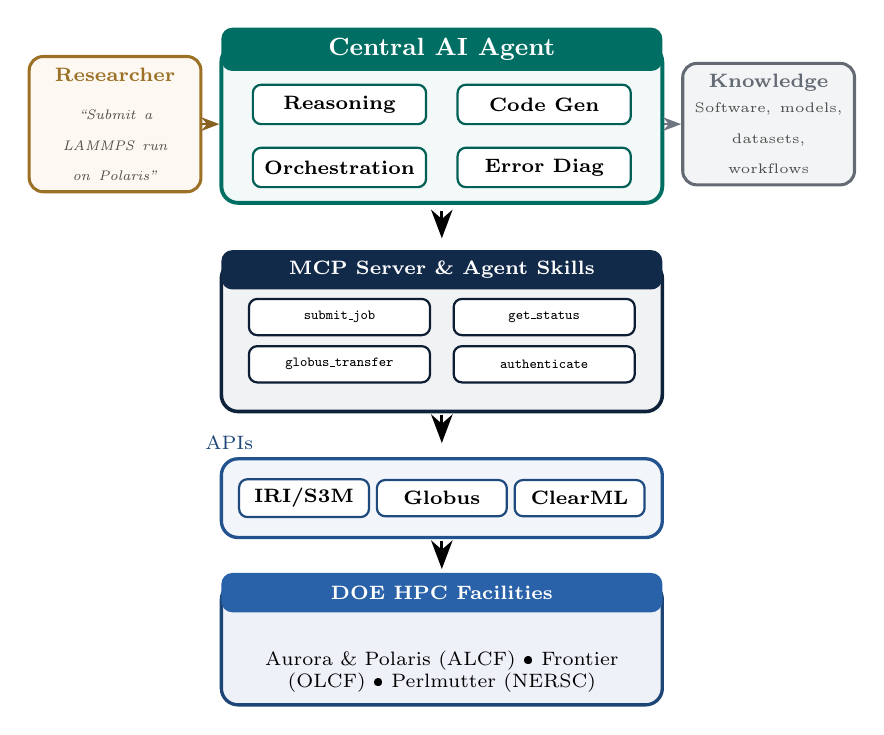
\begin{tikzpicture}[font=\small, line width=0.8pt]

      %% ---- Central AI Agent ----
      \node[draw=accentteal!80!black, fill=accentteal!5!white, rounded corners=6pt,
            minimum width=5.6cm, minimum height=2.0cm, line width=1.4pt]
            (agent) at (0,7.6) {};
      \node[fill=accentteal!80!black, text=white, rounded corners=4pt,
            minimum width=5.6cm, minimum height=0.55cm,
            font=\bfseries\small] at (0,8.55) {Central AI Agent};
      \foreach \px/\py/\lbl in {-1.3/7.85/Reasoning, 1.3/7.85/{Code Gen},
                                  -1.3/7.05/Orchestration, 1.3/7.05/{Error Diag}}{
        \node[draw=accentteal!70!black, fill=white, rounded corners=3pt,
              minimum width=2.2cm, minimum height=0.5cm, font=\bfseries\scriptsize]
              at (\px,\py) {\lbl};}
      \node[draw=accentgold!70!black, fill=accentgold!7!white, rounded corners=5pt, align=center,
            text width=1.9cm, inner sep=4pt, line width=1.1pt]
            (human) at (-4.15,7.6)
            {{\scriptsize\color{accentgold!70!black}\textbf{Researcher}}\\[3pt]
             \tiny\itshape\color{black!70} ``Submit a LAMMPS run on Polaris''};
      \draw[-{Stealth}, accentgold!60!black] (human.east) -- (agent.west);
      \node[draw=midgray!90!black, fill=midgray!8!white, rounded corners=5pt, align=center,
            text width=1.9cm, inner sep=4pt, line width=1.1pt]
            (know) at (4.15,7.6)
            {{\scriptsize\color{midgray!90!black}\textbf{Knowledge}}\\[3pt]
             \tiny\color{black!70} Software, models,\\datasets, workflows};
      \draw[-{Stealth}, midgray] (agent.east) -- (know.west);

      \draw[-{Stealth[scale=1.3]}, black, line width=1.1pt] (0,6.5) -- (0,6.15);

      %% ---- MCP row ----
      \node[draw=labnavy!80!black, fill=labnavy!6!white, rounded corners=6pt,
            minimum width=5.6cm, minimum height=1.9cm, line width=1.3pt] (mcp) at (0,4.9) {};
      \node[fill=labnavy, text=white, rounded corners=4pt,
            minimum width=5.6cm, minimum height=0.5cm,
            font=\bfseries\scriptsize] at (0,5.75) {MCP Server \& Agent Skills};
      \foreach \px/\py/\lbl in {-1.3/5.15/{submit\_job}, 1.3/5.15/{get\_status},
                                  -1.3/4.55/{globus\_transfer}, 1.3/4.55/{authenticate}}{
        \node[draw=labnavy!70!black, fill=white, rounded corners=3pt,
              minimum width=2.3cm, minimum height=0.46cm, font=\ttfamily\tiny]
              at (\px,\py) {\lbl};}

      \draw[-{Stealth[scale=1.3]}, black, line width=1.1pt] (0,3.9) -- (0,3.55);

      %% ---- APIs row ----
      \node[draw=accentblue!85!black, fill=accentblue!6!white, rounded corners=6pt,
            minimum width=5.6cm, minimum height=1.0cm, line width=1.2pt] (apis) at (0,2.85) {};
      \foreach \px/\lbl in {-1.75/{IRI/S3M},0/{Globus},1.75/{ClearML}}{
        \node[draw=accentblue!75!black, fill=white, rounded corners=3pt,
              minimum width=1.65cm, minimum height=0.46cm, font=\bfseries\scriptsize]
              at (\px,2.85) {\lbl};}
      \node[font=\scriptsize, text=accentblue!70!black] at (-2.7,3.55) {APIs};

      \draw[-{Stealth[scale=1.3]}, black, line width=1.1pt] (0,2.3) -- (0,1.95);

      %% ---- HPC facilities row ----
      \node[draw=accentblue!70!black, fill=accentblue!8!white, rounded corners=6pt,
            minimum width=5.6cm, minimum height=1.55cm, line width=1.2pt] (hpc) at (0,1.0) {};
      \node[fill=accentblue, text=white, rounded corners=4pt,
            minimum width=5.6cm, minimum height=0.5cm,
            font=\bfseries\scriptsize] at (0,1.65) {DOE HPC Facilities};
      \node[font=\scriptsize, align=center, text width=5.0cm] at (0,0.65)
           {Aurora \& Polaris (ALCF) \textbullet\ Frontier (OLCF) \textbullet\ Perlmutter (NERSC)};
      \end{tikzpicture}%
      }
      \end{center}
    \end{column}
    \begin{column}{0.03\textwidth}\end{column}
    \begin{column}{0.44\textwidth}
      \begin{featbox}{labnavy}{\faTasks\ Domains (600+ campaigns)}
        \begin{center}
        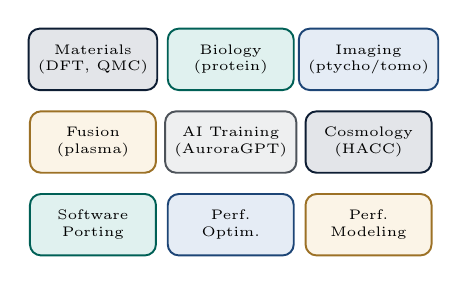
\begin{tikzpicture}[font=\tiny]
          \node[chip=labnavy]     at (-1.75, 0.55) {Materials\\(DFT, QMC)};
          \node[chip=accentteal]  at ( 0.00, 0.55) {Biology\\(protein)};
          \node[chip=accentblue]  at ( 1.75, 0.55) {Imaging\\(ptycho/tomo)};
          \node[chip=accentgold]  at (-1.75,-0.50) {Fusion\\(plasma)};
          \node[chip=midgray]     at ( 0.00,-0.50) {AI Training\\(AuroraGPT)};
          \node[chip=labnavy]     at ( 1.75,-0.50) {Cosmology\\(HACC)};
          \node[chip=accentteal]  at (-1.75,-1.55) {Software\\Porting};
          \node[chip=accentblue]  at ( 0.00,-1.55) {Perf.\\Optim.};
          \node[chip=accentgold]  at ( 1.75,-1.55) {Perf.\\Modeling};
        \end{tikzpicture}
        \end{center}
      \end{featbox}
      \par\vspace{4pt}
      {\scriptsize\itshape\color{midgray} 600+ autonomous campaigns across 13 DOE systems, 3 facilities --- domain agnostic.}
    \end{column}
  \end{columns}
\end{frame}

% ================================================================ TRINITY — LAMMPS EXAMPLE (trinity_overview.tex: "A plain-language request…")
\begin{frame}[fragile]{A plain-language request becomes a monitored PBS job}
  \begin{chatbubble}{accentgold}{\faUser\ Scientist}
    \scriptsize ``Submit a 4-node LAMMPS run on Polaris under my allocation, then let me know when it's done.''
  \end{chatbubble}
  \vspace{1pt}
  \begin{chatbubble}{accentteal}{\faRobot\ Trinity}
    \scriptsize Resolved account \& run directory via \texttt{run\_dir.py}, generated the job script below,
    and submitted it through the \texttt{submit-job} skill.
  \end{chatbubble}
  \vspace{1pt}
  \noindent\tikz[baseline]{\node[fill=labink, text=white, rounded corners=2pt,
    inner sep=2pt, font=\bfseries\tiny\ttfamily] {\faTerminal\ run.sh (bash)};}\par\vspace{0pt}
  \begin{lstlisting}[style=shell]
#!/bin/bash -l
#PBS -A <allocation> -q prod -l select=4:system=polaris -l walltime=01:00:00
WORKDIR="$(cd "$(dirname "$0")/.." && pwd)"; cd "$WORKDIR"
mpiexec -n 16 --ppn 4 lmp -in in.lammps   # -> outputs/, logs/
  \end{lstlisting}
  \vspace{1pt}
  \begin{tcolorbox}[enhanced, colback=accentteal!10, colframe=accentteal!60!black, boxrule=0.5pt,
    arc=4pt, left=6pt, right=6pt, top=2pt, bottom=2pt, width=\linewidth,
    drop fuzzy shadow]
    \scriptsize\faCheckCircle\ \textbf{Trinity:} Job \texttt{1234567} completed in 42 min on 4 Polaris nodes ---
    results saved under \texttt{jobs/polaris/lammps\_run/outputs/}.
  \end{tcolorbox}
\end{frame}

% ================================================================ TRINITY — AGENT HUB (trinity_overview.tex: "Agents and skills…")
\begin{frame}{Agents and skills are both discoverable, reusable catalogs}
  \begin{columns}[t, totalwidth=\textwidth]
    \begin{column}{0.47\textwidth}
      \begin{featbox}{accentteal}{\faRobot\ Agent Hub (A2A-aligned)}
        \scriptsize
        \begin{itemize}\itemsep1pt
          \item Standard agent card: profile, auth, query, skills, knowledge
          \item \texttt{/card} $\cdot$ \texttt{/token} $\cdot$ \texttt{/query} $\cdot$ \texttt{.well-known/agent-card}
          \item Third-party agents register and participate in rooms
          \item Query any agent via \texttt{POST /api/agents/\{id\}/query}
        \end{itemize}
      \end{featbox}
    \end{column}
    \begin{column}{0.06\textwidth}\end{column}
    \begin{column}{0.47\textwidth}
      \begin{featbox}{accentblue}{\faTools\ Skill \& Workflow Hub}
        \scriptsize
        \begin{itemize}\itemsep1pt
          \item Reusable workflow templates as versioned YAML cards
          \item Discoverable via \texttt{/api/workflows} (build-software, submit-job, \ldots)
          \item Scientists can define custom workflows and agents
          \item Shared, read-only catalog across all tenants
        \end{itemize}
      \end{featbox}
    \end{column}
  \end{columns}
  \vspace{2pt plus 1pt minus 2pt}
  \begin{center}
  \begin{tcolorbox}[enhanced, colback=labnavy!6, colframe=labnavy, boxrule=0.6pt,
    arc=3pt, width=0.9\linewidth, left=10pt, right=10pt, top=1pt, bottom=1pt,
    drop fuzzy shadow]
    \centering\footnotesize
    \faGithub\ \textbf{Community registry: Trinity Hub} --- publish an agent (A2A / OpenAI-chat / REST)
    or contribute a reusable skill via pull request.
  \end{tcolorbox}
  \end{center}
\end{frame}

% ================================================================ TRINITY — SHARED ROOMS (trinity_overview.tex: "Shared rooms…")
\begin{frame}{Shared rooms let humans and agents work in one conversation}
  \begin{columns}[t]
    \begin{column}{0.44\textwidth}
      \vspace{16pt}
      \small
      \begin{itemize}\itemsep10pt
        \item[\faComments] \textbf{Shared rooms} where humans and AI
          agents co-exist as first-class participants (\texttt{core/rooms.py})
        \item[\faBolt] \textbf{Every participant sees updates instantly}
          --- no refresh, no polling
        \item[\faUserShield] Agents run under \textbf{the owner's own
          tokens}, with a \textbf{budget gate the owner sets}
      \end{itemize}
    \end{column}
    \begin{column}{0.53\textwidth}
      \begin{tcolorbox}[enhanced, colback=lightgray!40!white, colframe=midgray!55,
        boxrule=0.8pt, arc=6pt, boxsep=0pt, left=6pt, right=6pt, top=4pt, bottom=5pt,
        width=\linewidth, drop fuzzy shadow,
        title={\tikz[baseline=-0.4ex]{\foreach \c/\dx in {red!70!black/0, orange!90!yellow/0.32, green!45!black/0.64}{\fill[\c] (\dx,0) circle (0.045);}}%
          \hspace{7pt}\#xrf-ptychography-2ide},
        colbacktitle=labink, coltitle=white, fonttitle=\bfseries\scriptsize]
      \begin{flushright}
      \begin{tcolorbox}[enhanced, colback=accentgold!15, colframe=accentgold!15, boxrule=0pt,
        arc=8pt, left=7pt, right=7pt, top=2pt, bottom=2pt, width=0.94\linewidth, boxsep=0pt]
        \scriptsize\color{labink}\textbf{\color{accentgold!70!black}\faUser\ huihuo.zheng:}
        Let's enhance the XRF map for Lamni-6 using the ptychographic probe.
      \end{tcolorbox}
      \end{flushright}
      \vspace{2pt}
      \begin{flushleft}
      \begin{tcolorbox}[enhanced, colback=accentblue!12, colframe=accentblue!12, boxrule=0pt,
        arc=8pt, left=7pt, right=7pt, top=2pt, bottom=2pt, width=0.94\linewidth, boxsep=0pt]
        \scriptsize\color{labink}\textbf{\color{accentblue!70!black}\faRobot\ super-ray:}
        @trinity --- transfer the data to Eagle, run the pipeline, send results back.
      \end{tcolorbox}
      \end{flushleft}
      \vspace{2pt}
      \begin{flushleft}
      \begin{tcolorbox}[enhanced, colback=accentteal!12, colframe=accentteal!12, boxrule=0pt,
        arc=8pt, left=7pt, right=7pt, top=2pt, bottom=2pt, width=0.94\linewidth, boxsep=0pt]
        \scriptsize\color{labink}\textbf{\color{accentteal!60!black}\faRobot\ trinity:}
        Data staged, pipeline complete --- +157.6\% sharpness on the Mn map.
      \end{tcolorbox}
      \end{flushleft}
      \vspace{2pt}
      \begin{flushright}
      \begin{tcolorbox}[enhanced, colback=accentgold!15, colframe=accentgold!15, boxrule=0pt,
        arc=8pt, left=7pt, right=7pt, top=2pt, bottom=2pt, width=0.94\linewidth, boxsep=0pt]
        \scriptsize\color{labink}\textbf{\color{accentgold!70!black}\faUser\ huihuo.zheng:}
        Great work --- write up a campaign report.
      \end{tcolorbox}
      \end{flushright}
      \end{tcolorbox}
    \end{column}
  \end{columns}
\end{frame}

% ================================================================ ACKNOWLEDGEMENT (from trinity_overview.tex)
\begin{frame}{Acknowledgement}
  \vspace{10pt}
  \small
  This research used resources of the \textbf{Argonne Leadership Computing
  Facility (ALCF)} at Argonne National Laboratory (Contract No.\
  DE-AC02-06CH11357), the \textbf{Oak Ridge Leadership Computing Facility
  (OLCF)} at Oak Ridge National Laboratory (Contract No.\
  DE-AC05-00OR22725), and the \textbf{National Energy Research Scientific
  Computing Center (NERSC)} (award ALCC-ERCAP0038560) --- all DOE Office
  of Science user facilities.
  \vspace{18pt}
  \begin{center}
  \begin{tcolorbox}[enhanced, colback=labnavy!6, colframe=labnavy, boxrule=0.6pt,
    arc=3pt, width=0.7\linewidth, left=12pt, right=12pt, top=8pt, bottom=8pt,
    drop fuzzy shadow]
    \begin{minipage}[c]{0.16\linewidth}
      \centering
      \begin{tikzpicture}
        \clip (0,0) circle (0.55cm);
        \node at (0,0) {\includegraphics[width=1.1cm]{yi_jiang.jpg}};
      \end{tikzpicture}
    \end{minipage}%
    \begin{minipage}[c]{0.8\linewidth}
      \small Special thanks to \textbf{Yi Jiang} (Advanced Photon Source)
      for many fruitful, inspiring discussions.
    \end{minipage}
  \end{tcolorbox}
  \end{center}
\end{frame}

\end{document}
